\begin{figure}[htbp]
\section*{ANKRD11}
\centering
\begin{subfigure}[b]{0.95\textwidth}
\centering
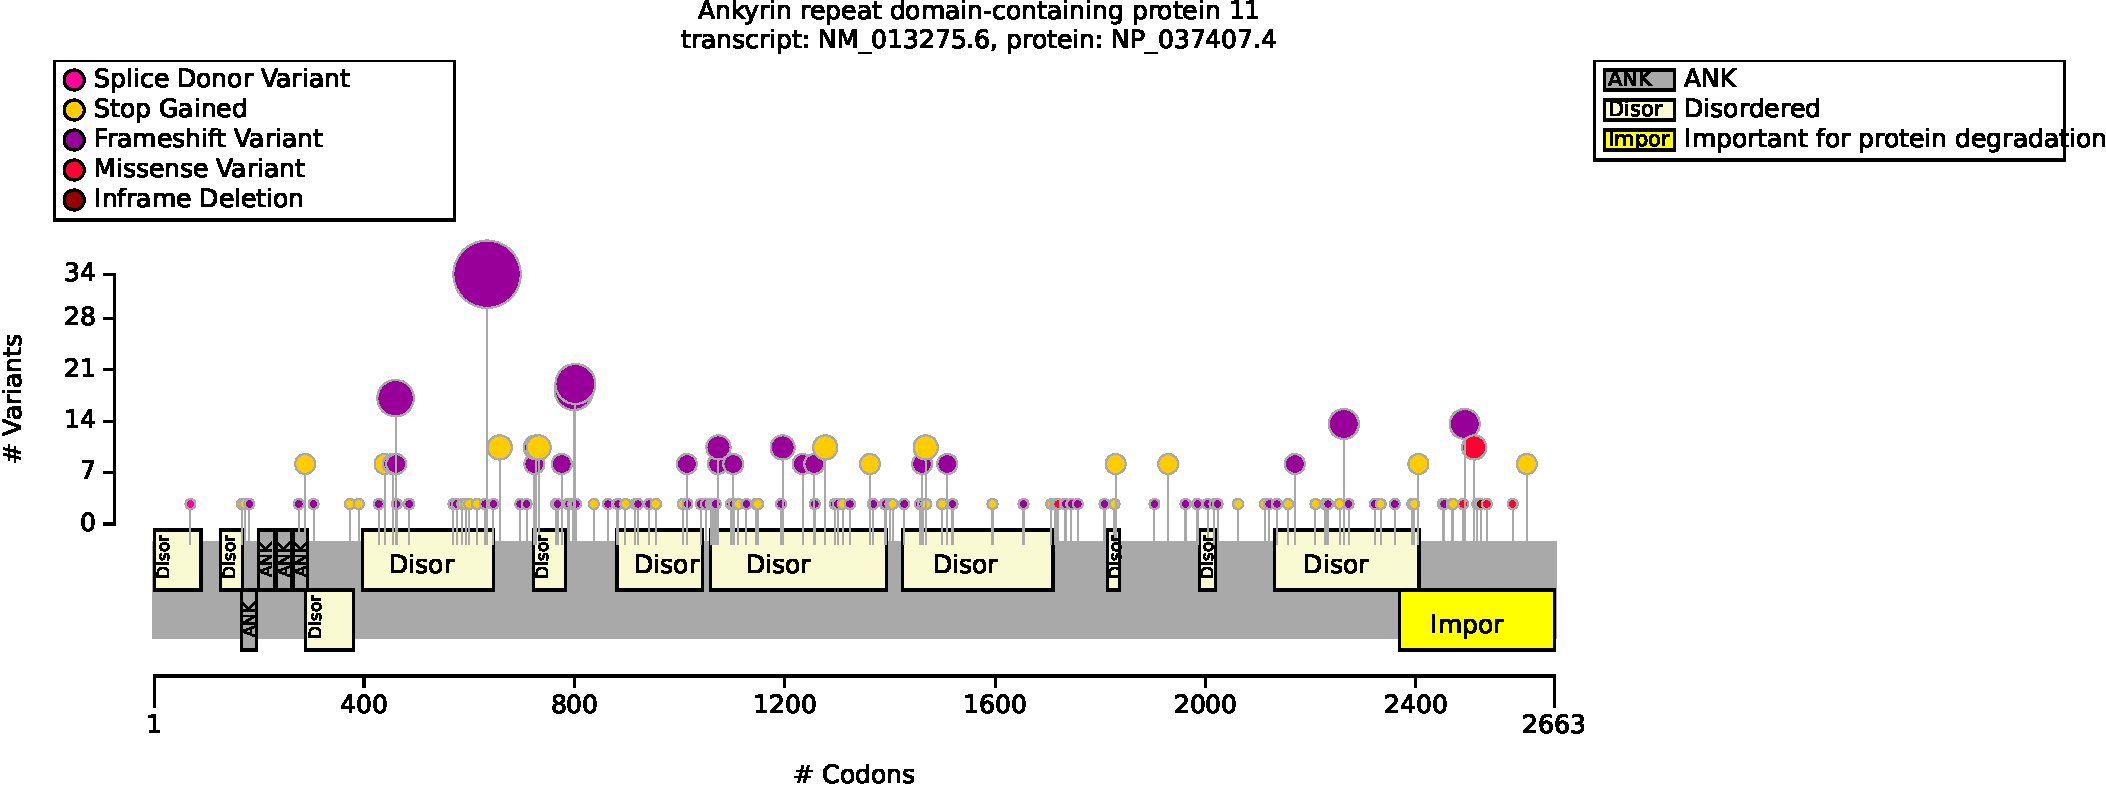
\includegraphics[width=\textwidth]{ img/ANKRD11_protein_diagram.pdf} 
\captionsetup{justification=raggedright,singlelinecheck=false}
\caption{Distribution of variants in ANKRD11}
\end{subfigure}

\vspace{2em}

\begin{subfigure}[b]{0.95\textwidth}
\centering
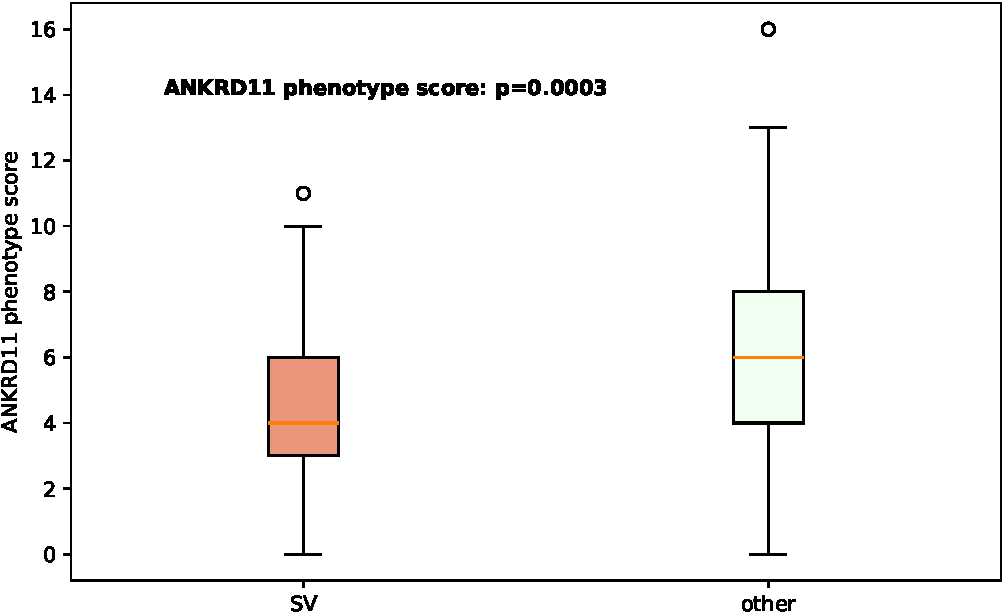
\includegraphics[width=0.3\textwidth]{ img/ANKRD11_phenoscore.pdf} 
\captionsetup{justification=raggedright,singlelinecheck=false}
\caption{ANKRD11 phenotypical score. Mean for structural variants: 4.62, and for other variants: 5.94}
\end{subfigure}

\vspace{2em}

\begin{subfigure}[b]{0.95\textwidth}
\centering
\resizebox{\textwidth}{!}{
\begin{tabular}{llllrr}
\toprule
Genotype (A) & Genotype (B) & total tests performed & significant results\\
\midrule
SV & other & 17 & 0\\
exon 9 & other & 17 & 0\\
c.1903\_1907del & other & 17 & 0\\
\bottomrule
\end{tabular}
}
\captionsetup{justification=raggedright,singlelinecheck=false}
\caption{Fisher Exact Test performed to compare HPO annotation frequency with respect to SV, exon 9, and c.1903\_1907del.}
\end{subfigure}

\vspace{2em}

\begin{subfigure}[b]{0.95\textwidth}
\captionsetup{justification=raggedright,singlelinecheck=false}
\resizebox{\textwidth}{!}{
\begin{tabular}{llllrr}
\toprule
Description & Variable & Genotype (A) & Genotype (B) & p-value & xrefs\\
\midrule
ANKRD11 phenotype score & HPO group count & SV & other & $2.64\times 10^{-4}$ & \cite{PMID_36446582}\\
ANKRD11 phenotype score & HPO group count & FEMALE & MALE & 0.0075 & -\\

\bottomrule
\end{tabular}
}
\caption{AKKRD11 phenotype score for structural variants: 4.62; other variants: 5.94. male/female comparison: Female 5.28, Male: 6.15.}
\end{subfigure}

\vspace{2em}

\caption{The cohort comprised 337 individuals (143 females, 175 males, 19 with unknown sex). A total of 48 HPO terms were used to annotate the cohort. Disease diagnosis: KBG syndrome (OMIM:148050). Validated results on ANKRD11 phenotypical score. Other results did not survive multiple testing correction. A total of 337 unique variant alleles were found in \textit{ANKRD11} (transcript: \texttt{NM\_013275.6}, protein id: \texttt{NP\_037407.4}).}
\end{figure}
